\chapter{Results}\label{chp:results}
%\section{Results}\label{sec:Results}

This section presents the simulations we performed to evaluate the
proposed test statistics' performance, followed by applications to SAR
data.

\section{Simulated Data}\label{simulated-data}

Figure~\ref{fig:sim_Phantom} \ref{fig:sim_Phantom_1} shows the phantom with dimensions of
\(500\times500\) pixels.
 It was proposed by~\citet{Gomez2017} as a tool
to assess the performance of speckle-reduction filters.

Figure~\ref{fig:sim_Phantom} \ref{fig:sim_Phantom_2} shows the simulated image, where each
small phantom displaying texture variations. The observations are
independent draws from the \(G^0_I\) distribution~\eqref{E:gi02}, with
\(L = 5\) and varying \(\alpha\) and \(\mu\), annotated in the image for
each quadrant. 
Light regions correspond to textured observations
(heterogeneous), while darker regions represent textureless areas
(homogeneous).
\begin{figure}[H]
  \centering
  \begin{subfigure}[b]{0.38\textwidth}
    \centering
    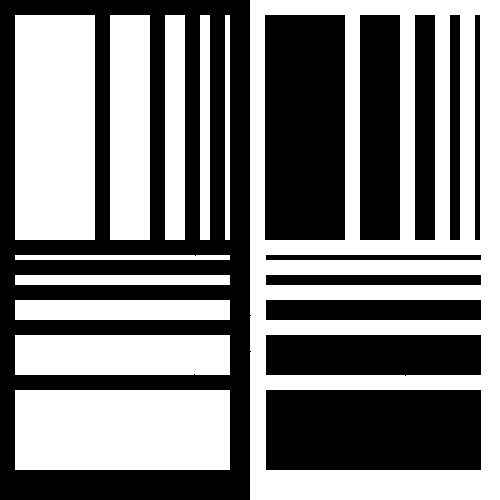
\includegraphics[width=60mm]{../../Figures/PNG/Phantom1}
    \caption{Phantom.}
    \label{fig:sim_Phantom_1}
  \end{subfigure}
  \hfill
  \begin{subfigure}[b]{0.58\textwidth}
    \centering
    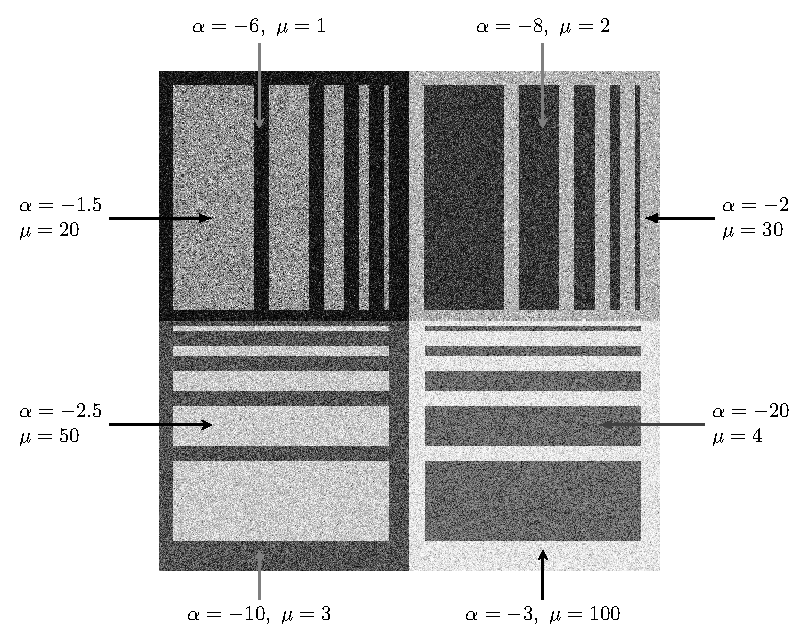
\includegraphics[width=80mm]{../../Figures/PNG/Phantom_label/Phantom_labels}
    \caption{Simulated image, varying $\alpha$ and $\mu$, with $L=5$.}
    \label{fig:sim_Phantom_2}
  \end{subfigure}
  \caption{Synthetic dataset.}
  \label{fig:sim_Phantom}
\end{figure}


The \(\alpha\) parameter of the \(G_I^0\) distribution is essential for
interpreting texture characteristics. Values near zero greater than
\(-3\) suggest extremely textured targets, such as urban
zones~\citep{Frery2019a}. 
As the value decreases, it indicates regions with moderate texture (in the \(\left[-6,-3\right]\) region), related to
forest zones, while values below \(-6\) correspond to textureless
regions, such as pasture, agricultural fields, and water
bodies~\citep{Neto2023}.




We applied the three test statistics, namely
\(S_{\widetilde{H}_{\text{AO}}}(\bm{Z}; L)\), \(T_\text{CV}\), and
\(T_{\text{CV}_{\text{MnAD}}}\), to the simulated image using local
sliding windows of size \(7\times 7\), as shown in
Figures~\ref{fig:sim_results} \ref{fig:sim_results-1}--\ref{fig:sim_results-3}.
\begin{figure}[H]
  \centering
  \begin{subfigure}[b]{0.3\textwidth}
    \centering
    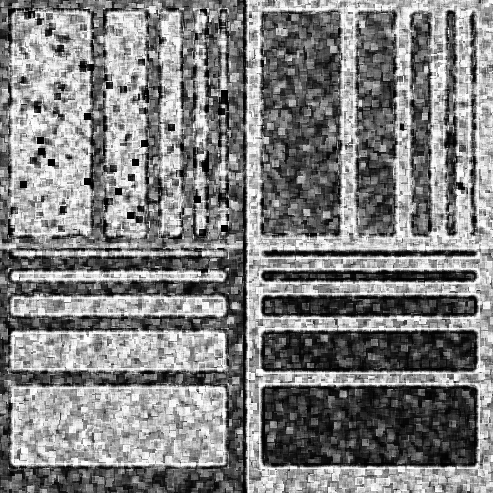
\includegraphics[width=\textwidth]{../../Figures/PNG/Entropy_Phantom_4_z1_200}
    \caption{$S_{\widetilde{H}_{\text{AO}}}(\bm{Z}; L)$}
    \label{fig:sim_results-1}
  \end{subfigure}
  \hfill
  \begin{subfigure}[b]{0.3\textwidth}
    \centering
    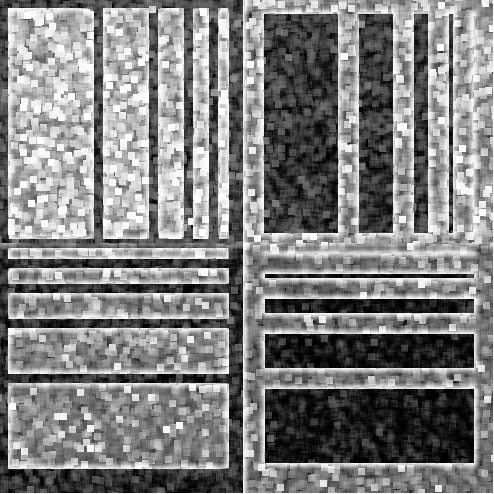
\includegraphics[width=\textwidth]{../../Figures/PNG/cv_Phantom_4_z1}
    \caption{$T_\text{CV}$}
    \label{fig:sim_results-2}
  \end{subfigure}
  \hfill
  \begin{subfigure}[b]{0.3\textwidth}
    \centering
    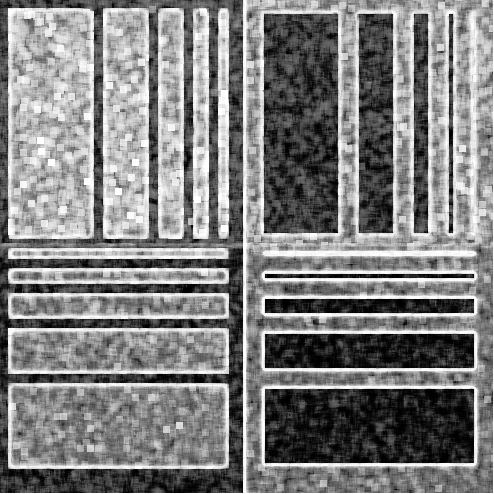
\includegraphics[width=\textwidth]{../../Figures/PNG/mnad_Phantom_z1}
    \caption{$T_{\text{CV}_{\text{MnAD}}}$}
    \label{fig:sim_results-3}
  \end{subfigure}
  \caption{Results of applying the test statistics to the simulated image.}
  \label{fig:sim_results}
\end{figure}



The resulting \(p\)-values for each test are shown in
Figures~\ref{fig:sim_SAR_Images} \ref{fig:sim_SAR_Images-1}--\ref{fig:sim_SAR_Images-3}. In
Figures~\ref{fig:sim_SAR_Images_p05} \ref{fig:sim_SAR_Images_p05-1}--\ref{fig:sim_SAR_Images_p05-3}, maps are depicted using a
color table between black, gray levels, and white. All \(p\)-values
above \(0.05\) are represented in white (indicating no evidence to
reject the null hypothesis), while those below \(0.05\) are shown in
black (indicating evidence to reject the hypothesis). 
We notice that the \(S_{\widetilde{H}_{\text{AO}}}(\bm{Z}; L)\) performs significantly
better than the other tests in identifying heterogeneous areas in the
simulated image.

\begin{figure}[H]
  \centering
  \begin{subfigure}[b]{0.3\textwidth}
    \centering
    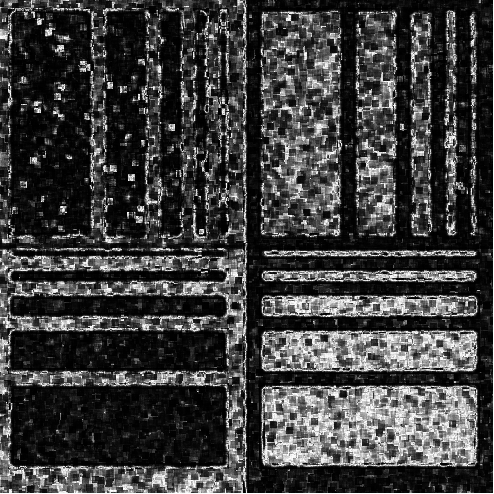
\includegraphics[width=\textwidth]{../../Figures/PNG/H_pvalue_Phantom_4_z1_200b}
    \caption{$S_{\widetilde{H}_{\text{AO}}}(\bm{Z}; L)$}
    \label{fig:sim_SAR_Images-1}
  \end{subfigure}
  \hfill
  \begin{subfigure}[b]{0.3\textwidth}
    \centering
    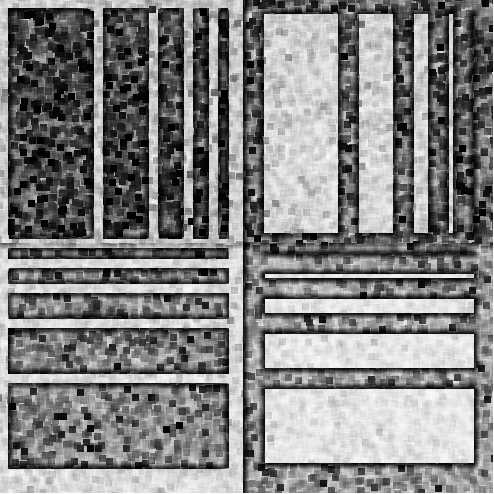
\includegraphics[width=\textwidth]{../../Figures/PNG/cv_pvalues_Phantom_4_z1}
    \caption{$T_\text{CV}$}
    \label{fig:sim_SAR_Images-2}
  \end{subfigure}
  \hfill
  \begin{subfigure}[b]{0.3\textwidth}
    \centering
    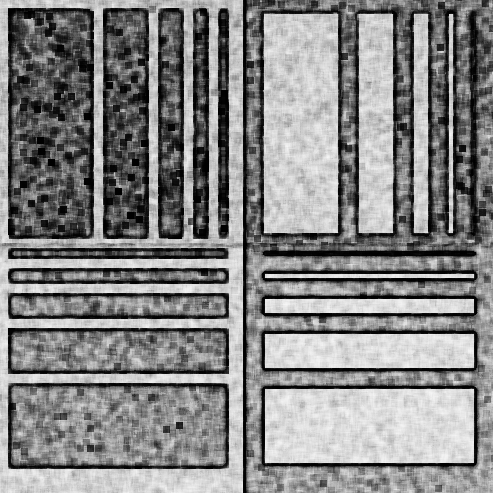
\includegraphics[width=\textwidth]{../../Figures/PNG/mnad_p_values_Phantom_mnad_7_z1}
     \caption{$T_{\text{CV}_{\text{MnAD}}}$}
    \label{fig:sim_SAR_Images-3}
  \end{subfigure}
  \caption{Map of $p$-values of simulated image for each test. }
  \label{fig:sim_SAR_Images}
\end{figure}



\begin{figure}[H]
  \centering
  \begin{subfigure}[b]{0.3\textwidth}
    \centering
    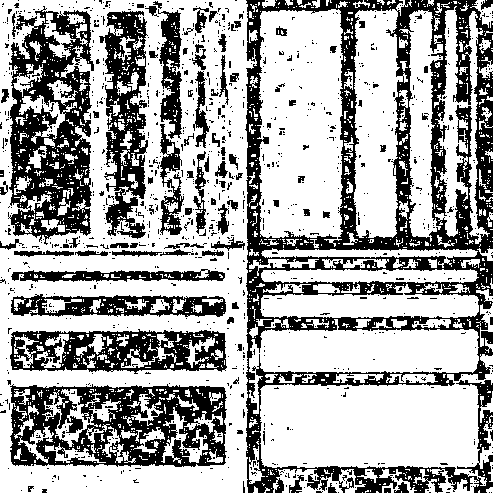
\includegraphics[width=\textwidth]{../../Figures/PNG/H_005_Phantom_4_z1_AO_200b}
    \caption{$S_{\widetilde{H}_{\text{AO}}}(\bm{Z}; L)$}
    \label{fig:sim_SAR_Images_p05-1}
  \end{subfigure}
  \hfill
  \begin{subfigure}[b]{0.3\textwidth}
    \centering
    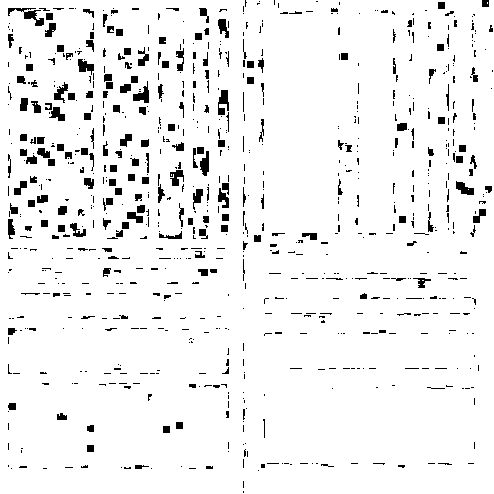
\includegraphics[width=\textwidth]{../../Figures/PNG/cv_005_pvalues_Phantom_4_z1}
    \caption{$T_\text{CV}$}
    \label{fig:sim_SAR_Images_p05-2}
  \end{subfigure}
  \hfill
  \begin{subfigure}[b]{0.3\textwidth}
    \centering
    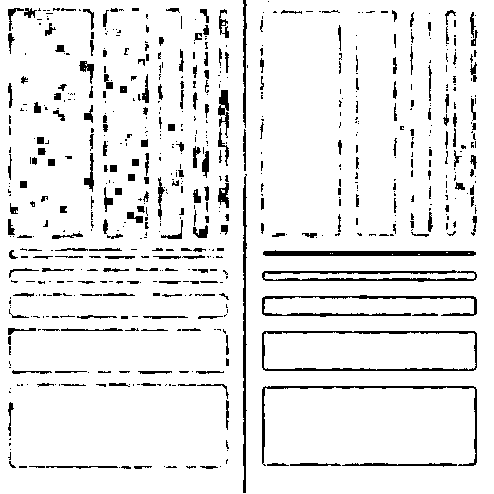
\includegraphics[width=\textwidth]{../../Figures/PNG/mnad_005_Phantom_7_z1}
     \caption{$T_{\text{CV}_{\text{MnAD}}}$}
    \label{fig:sim_SAR_Images_p05-3}
  \end{subfigure}
  \caption{Results for a threshold of $0.05$ of the $p$-value of simulated image for each test. }
  \label{fig:sim_SAR_Images_p05}
\end{figure}




\section{SAR Data}\label{sar-data}

We evaluated the proposed test statistics using three SAR images: one of
the coast of Jalisco, Mexico (with a spatial resolution of 20 m both
along azimuth and range directions) and two of Illinois, USA (with a
spatial resolution of \SI{10}{\meter} both along azimuth and range
directions), acquired by the Sentinel-1B satellite operating in C-band,
with VV polarization and intensity format. 
The first two images have a size of \(512 \times 512\) pixels, while the third has
\(1024 \times 1024\) pixels, and they contain mountainous areas,
agricultural regions, water bodies, and urban areas, as shown in
Figures~\ref{fig:real_SAR_Images_coe} \ref{fig:real_SAR_Images_coe-1}--\ref{fig:real_SAR_Images_coe-3}.

\begin{figure}[H]
  \centering
  \begin{subfigure}[b]{0.3\textwidth}
    \centering
    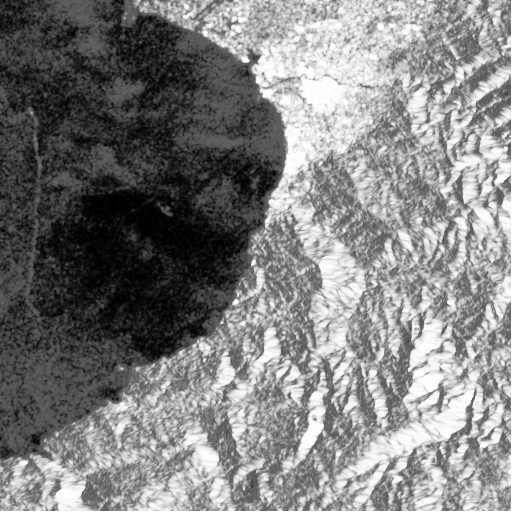
\includegraphics[width=\textwidth]{../../Figures/PNG/Mexico_512}
    \caption{Coast of Jalisco, $L=18$}
    \label{fig:real_SAR_Images_coe-1}
  \end{subfigure}
  \hfill
  \begin{subfigure}[b]{0.3\textwidth}
    \centering
    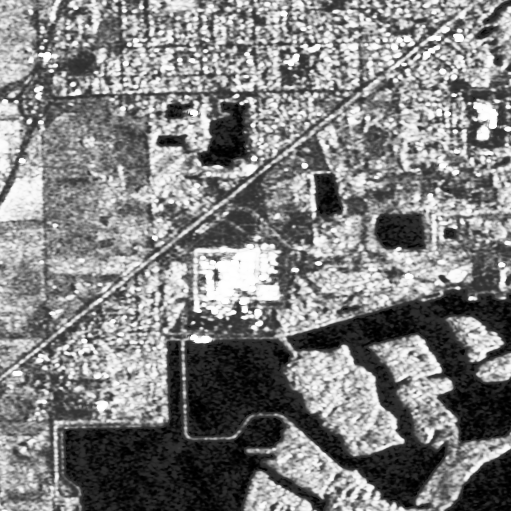
\includegraphics[width=\textwidth]{../../Figures/PNG/lake_512}
    \caption{Illinois-Region 1, $L=36$}
    \label{fig:real_SAR_Images_coe-2}
  \end{subfigure}
  \hfill
  \begin{subfigure}[b]{0.3\textwidth}
    \centering
    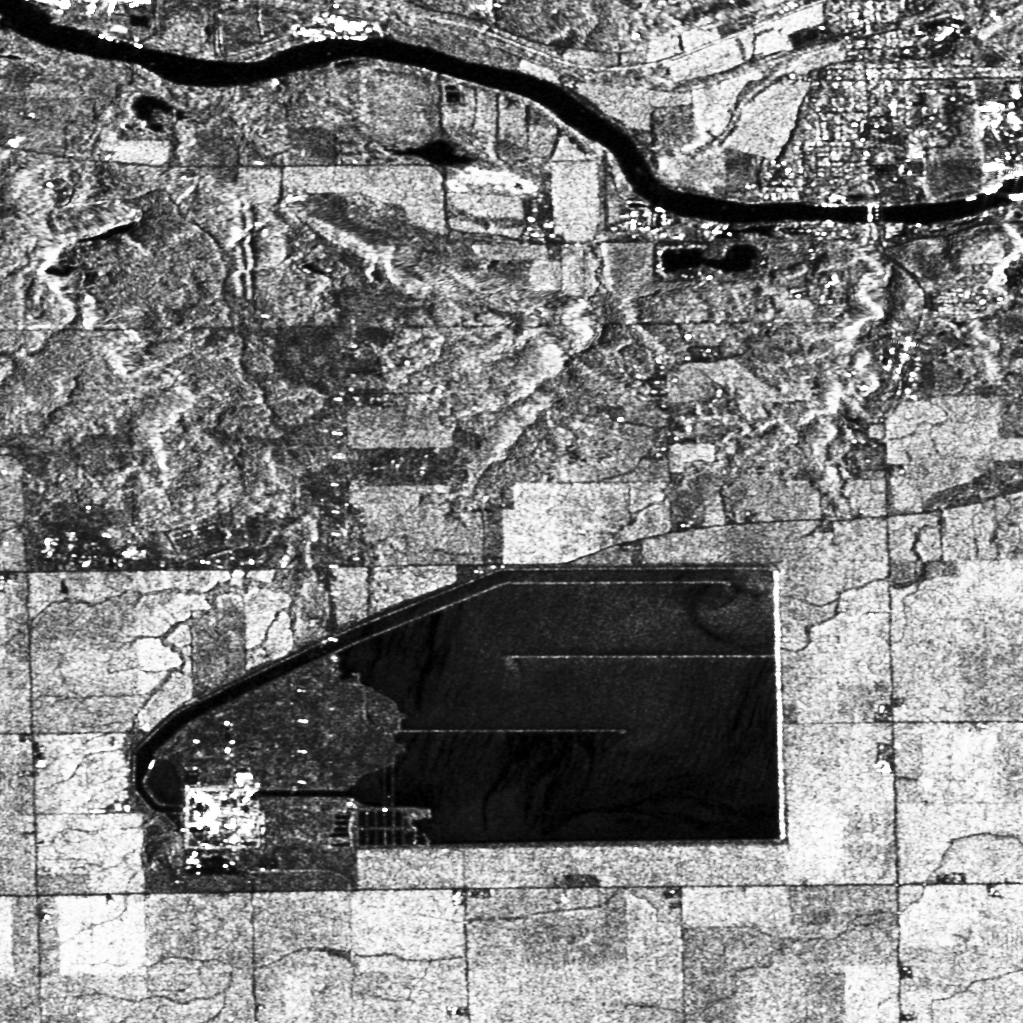
\includegraphics[width=\textwidth]{../../Figures/PNG/Illinois_1024_36L}
     \caption{Illinois-Region 2,  $L=36$}
    \label{fig:real_SAR_Images_coe-3}
  \end{subfigure}
  \caption{SAR images. }
  \label{fig:real_SAR_Images_coe}
\end{figure}



The three statistical tests are applied to the SAR images using
\(7\times 7\) local sliding windows, as illustrated in
Figures~\ref{fig:real_images_test_Mexico}, \ref{fig:test_lake}
and~\ref{fig:real_images_test_Illinois}.

The \(p\)-values obtained for each test are presented in
Figures~\ref{fig:Mexico_pvalue}, \ref{fig:lake_pvalue}
and~\ref{fig:Illinois_crops_pvalue}, respectively.

In Figures~\ref{fig:Mexico_crops_0.05}, \ref{fig:lake_0.05}
and~\ref{fig:Illinois_crops_0.05}, the maps of \(p\)-values composed of
a linear gradient of black and white colors, represent the decisions at
a \SI{5}{\percent} significance level.
Dark areas represent values below
\(0.05\), indicating evidence to reject the null hypothesis and
suggesting heterogeneity in these regions. 
In contrast, values above 0.05 are represented as white areas, indicating no evidence to reject
the fully-developed speckle hypothesis.
\begin{figure}[H]
  \centering
  \begin{subfigure}[b]{0.3\textwidth}
    \centering
    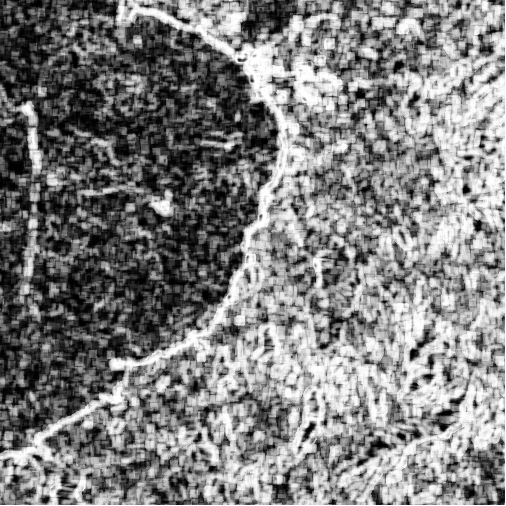
\includegraphics[width=\textwidth]{../../Figures/PNG/Entropy_Mexico_512_18L_AO_200b}
    \caption{$S_{\widetilde{H}_{\text{AO}}}(\bm{Z}; L)$}
    \label{fig:real_images_test_Mexico-1}
  \end{subfigure}
  \hfill
  \begin{subfigure}[b]{0.3\textwidth}
    \centering
    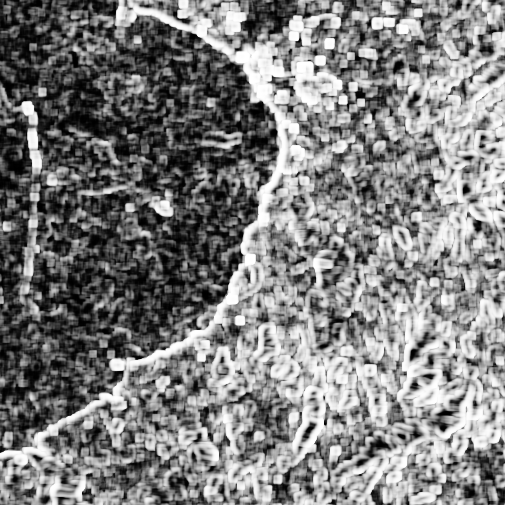
\includegraphics[width=\textwidth]{../../Figures/PNG/cv_mexico_512}
    \caption{$T_\text{CV}$}
    \label{fig:real_images_test_Mexico-2}
  \end{subfigure}
  \hfill
  \begin{subfigure}[b]{0.3\textwidth}
    \centering
    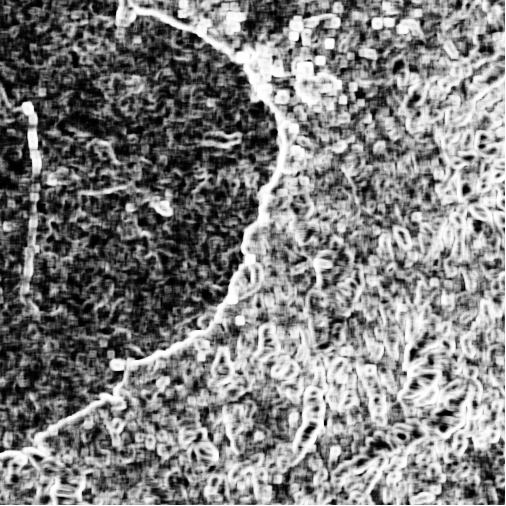
\includegraphics[width=\textwidth]{../../Figures/PNG/mnad_mexico_512}
    \caption{$T_{\text{CV}_{\text{MnAD}}}$}
    \label{fig:real_images_test_Mexico-3}
  \end{subfigure}
  \caption{Results of applying the test statistics to Coast of Jalisco image.}
  \label{fig:real_images_test_Mexico}
\end{figure}



\begin{figure}[H]
  \centering
  \begin{subfigure}[b]{0.3\textwidth}
    \centering
    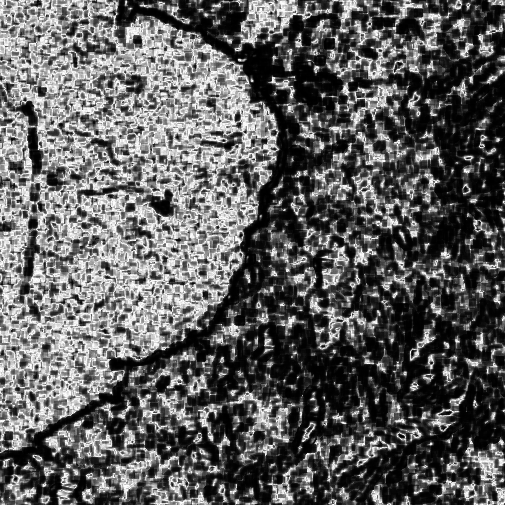
\includegraphics[width=\textwidth]{../../Figures/PNG/H_pvalue_Mexico_512_18L_AO_200b}
    \caption{$S_{\widetilde{H}_{\text{AO}}}(\bm{Z}; L)$}
    \label{fig:Mexico_pvalue-1}
  \end{subfigure}
  \hfill
  \begin{subfigure}[b]{0.3\textwidth}
    \centering
    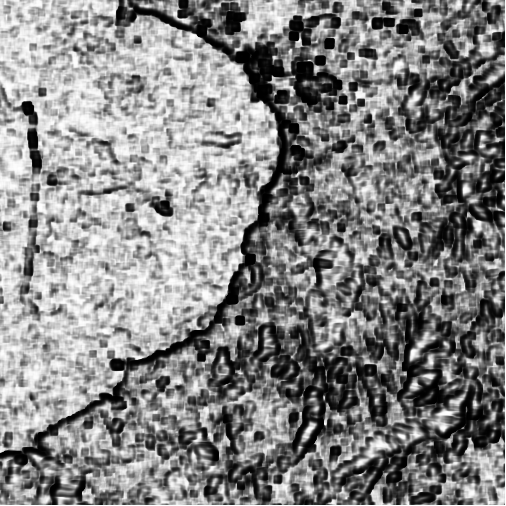
\includegraphics[width=\textwidth]{../../Figures/PNG/cv_pvalues_mexico_512}
    \caption{$T_\text{CV}$}
    \label{fig:Mexico_pvalue-2}
  \end{subfigure}
  \hfill
  \begin{subfigure}[b]{0.3\textwidth}
    \centering
    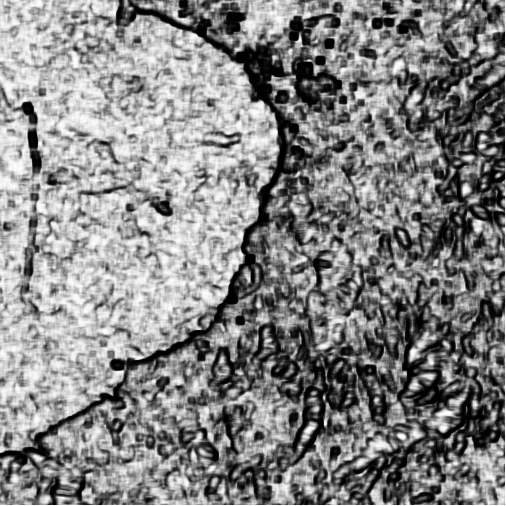
\includegraphics[width=\textwidth]{../../Figures/PNG/mnad_p_values_mexico_512}
     \caption{$T_{\text{CV}_{\text{MnAD}}}$}
    \label{fig:Mexico_pvalue-3}
  \end{subfigure}
  \caption{Map of $p$-values of Coast of Jalisco image for each test. }
  \label{fig:Mexico_pvalue}
\end{figure}



\begin{figure}[H]
  \centering
  \begin{subfigure}[b]{0.3\textwidth}
    \centering
    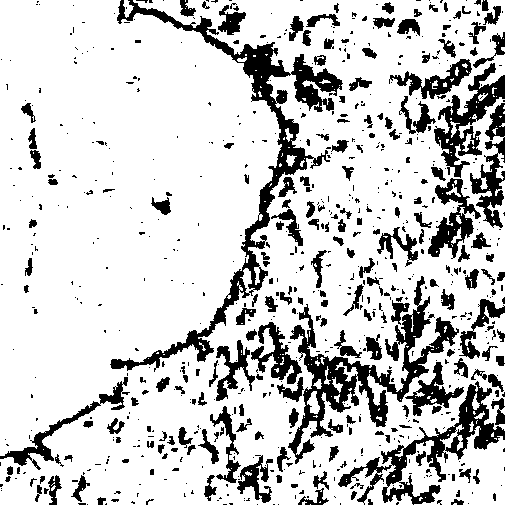
\includegraphics[width=\textwidth]{../../Figures/PNG/H_005__Mexico_512_18L_AO_200b}
    \caption{$S_{\widetilde{H}_{\text{AO}}}(\bm{Z}; L)$}
    \label{fig:Mexico_crops_0.05-1}
  \end{subfigure}
  \hfill
  \begin{subfigure}[b]{0.3\textwidth}
    \centering
    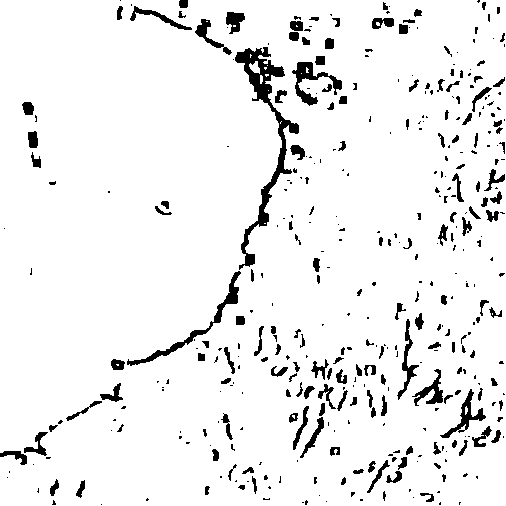
\includegraphics[width=\textwidth]{../../Figures/PNG/cv_005_pvalues_mexico_512}
    \caption{$T_\text{CV}$}
    \label{fig:Mexico_crops_0.05-2}
  \end{subfigure}
  \hfill
  \begin{subfigure}[b]{0.3\textwidth}
    \centering
    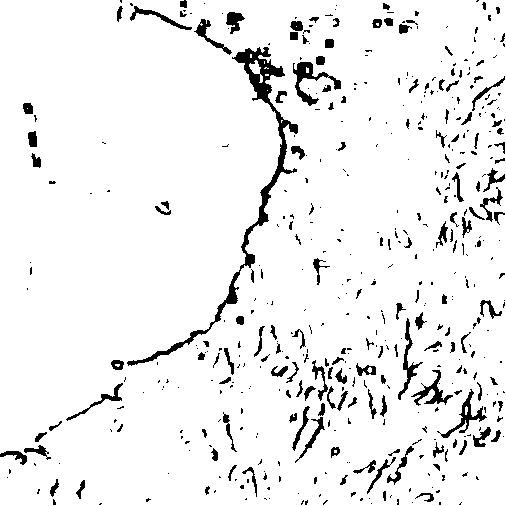
\includegraphics[width=\textwidth]{../../Figures/PNG/mnad_005_mexico_512}
     \caption{$T_{\text{CV}_{\text{MnAD}}}$}
    \label{fig:Mexico_crops_0.05-3}
  \end{subfigure}
  \caption{Results for a threshold of $0.05$ of the $p$-value of Coast of Jalisco for each test. }
  \label{fig:Mexico_crops_0.05}
\end{figure}



\begin{figure}[H]
  \centering
  \begin{subfigure}[b]{0.3\textwidth}
    \centering
    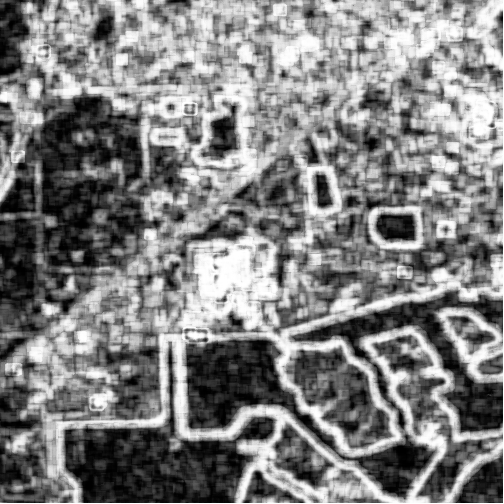
\includegraphics[width=\textwidth]{../../Figures/PNG/Entropy_lake_512_36L_AO_100b}
    \caption{$S_{\widetilde{H}_{\text{AO}}}(\bm{Z}; L)$}
    \label{fig:test_lake-1}
  \end{subfigure}
  \hfill
  \begin{subfigure}[b]{0.3\textwidth}
    \centering
    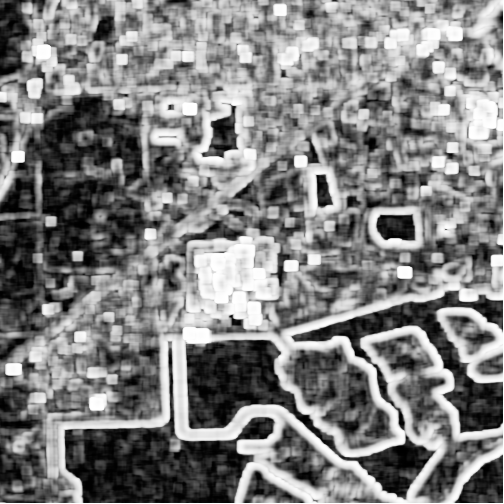
\includegraphics[width=\textwidth]{../../Figures/PNG/cv_lake_512}
    \caption{$T_\text{CV}$}
    \label{fig:test_lake-2}
  \end{subfigure}
  \hfill
  \begin{subfigure}[b]{0.3\textwidth}
    \centering
    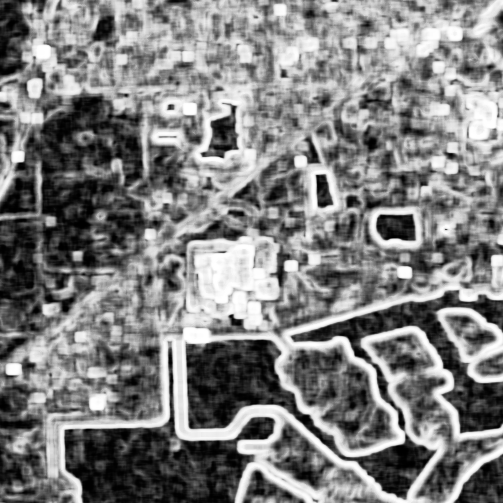
\includegraphics[width=\textwidth]{../../Figures/PNG/mnad_lake_512}
    \caption{$T_{\text{CV}_{\text{MnAD}}}$}
    \label{fig:test_lake-3}
  \end{subfigure}
  \caption{Results of applying the test statistics, Illinois-Region 1.}
  \label{fig:test_lake}
\end{figure}



\begin{figure}[H]
  \centering
  \begin{subfigure}[b]{0.3\textwidth}
    \centering
    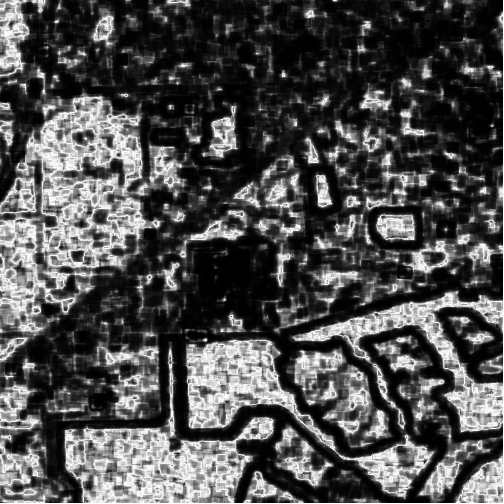
\includegraphics[width=\textwidth]{../../Figures/PNG/H_pvalue_lake_512_36L_AO_100b}
    \caption{$S_{\widetilde{H}_{\text{AO}}}(\bm{Z}; L)$}
    \label{fig:lake_pvalue-1}
  \end{subfigure}
  \hfill
  \begin{subfigure}[b]{0.3\textwidth}
    \centering
    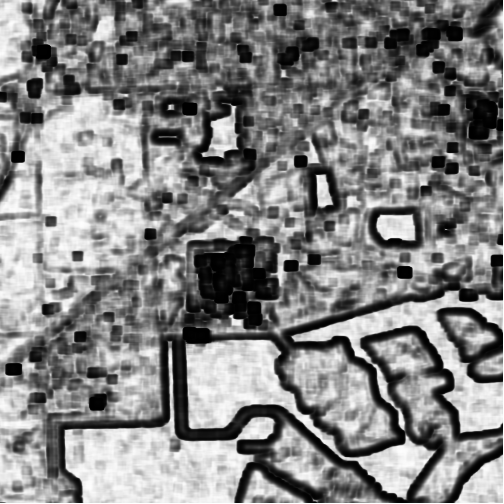
\includegraphics[width=\textwidth]{../../Figures/PNG/cv_pvalues_lake_512}
    \caption{$T_\text{CV}$}
    \label{fig:lake_pvalue-2}
  \end{subfigure}
  \hfill
  \begin{subfigure}[b]{0.3\textwidth}
    \centering
    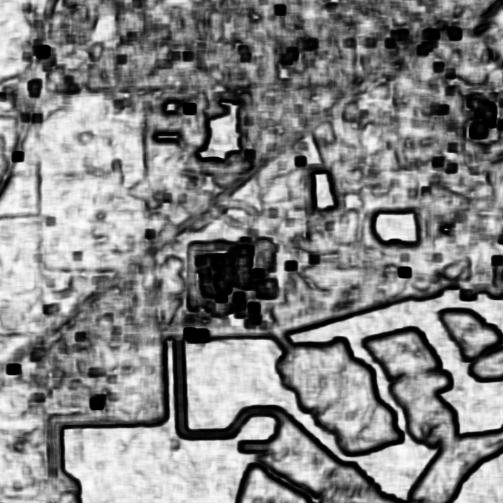
\includegraphics[width=\textwidth]{../../Figures/PNG/mnad_p_values_lake_512}
     \caption{$T_{\text{CV}_{\text{MnAD}}}$}
    \label{fig:lake_pvalue-3}
  \end{subfigure}
  \caption{Map of $p$-values, Illinois-Region 1. }
  \label{fig:lake_pvalue}
\end{figure}



\begin{figure}[H]
  \centering
  \begin{subfigure}[b]{0.3\textwidth}
    \centering
    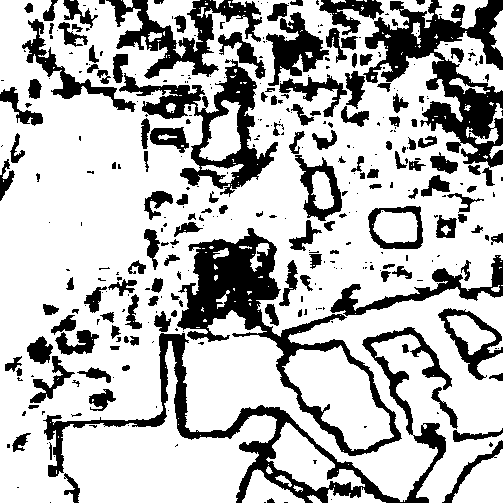
\includegraphics[width=\textwidth]{../../Figures/PNG/H_005_lake_512_36L_AO_100b}
    \caption{$S_{\widetilde{H}_{\text{AO}}}(\bm{Z}; L)$}
    \label{fig:lake_0.05-1}
  \end{subfigure}
  \hfill
  \begin{subfigure}[b]{0.3\textwidth}
    \centering
    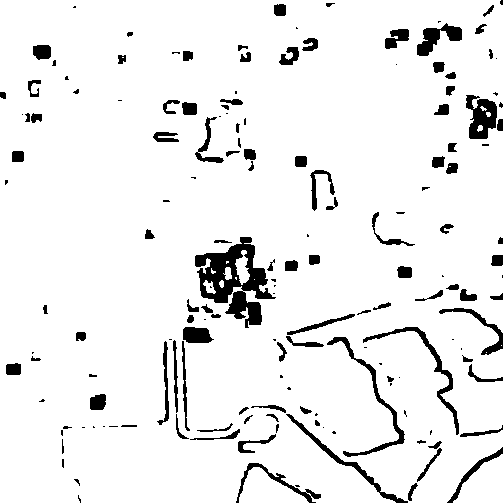
\includegraphics[width=\textwidth]{../../Figures/PNG/cv_005_pvalues_lake_512}
    \caption{$T_\text{CV}$}
    \label{fig:lake_0.05-2}
  \end{subfigure}
  \hfill
  \begin{subfigure}[b]{0.3\textwidth}
    \centering
    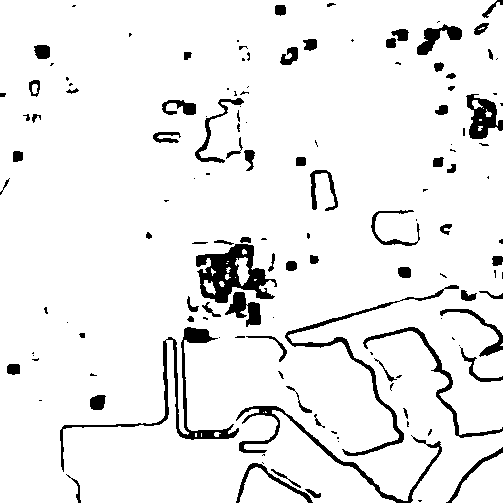
\includegraphics[width=\textwidth]{../../Figures/PNG/mnad_005_lake_512}
     \caption{$T_{\text{CV}_{\text{MnAD}}}$}
    \label{fig:lake_0.05-3}
  \end{subfigure}
  \caption{Results for a threshold of $0.05$ of the $p$-value, Illinois-Region 1. }
  \label{fig:lake_0.05}
\end{figure}




\begin{figure}[H]
  \centering
  \begin{subfigure}[b]{0.3\textwidth}
    \centering
    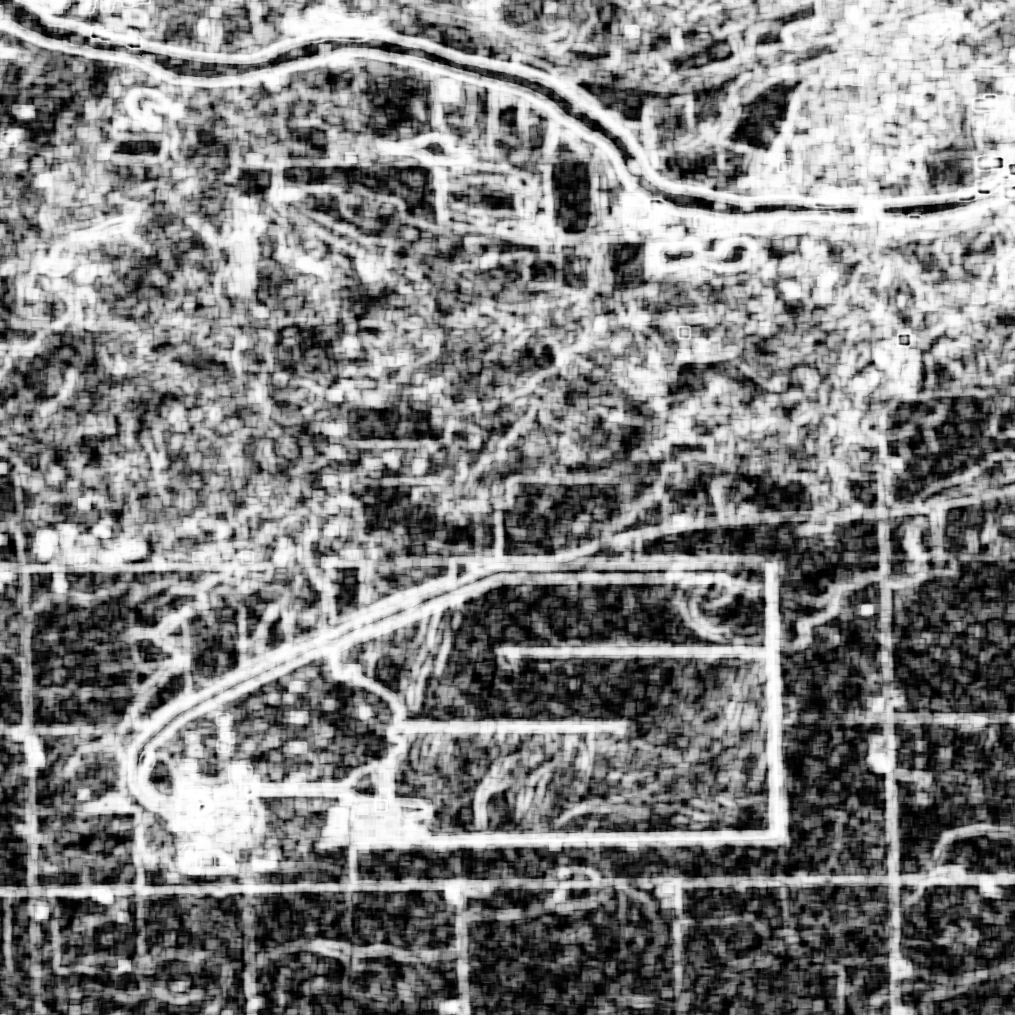
\includegraphics[width=\textwidth]{../../Figures/PNG/Entropy_Illinois_1024_36L_AO_200b}
    \caption{$S_{\widetilde{H}_{\text{AO}}}(\bm{Z}; L)$}
    \label{fig:real_images_test_Illinois-1}
  \end{subfigure}
  \hfill
  \begin{subfigure}[b]{0.3\textwidth}
    \centering
    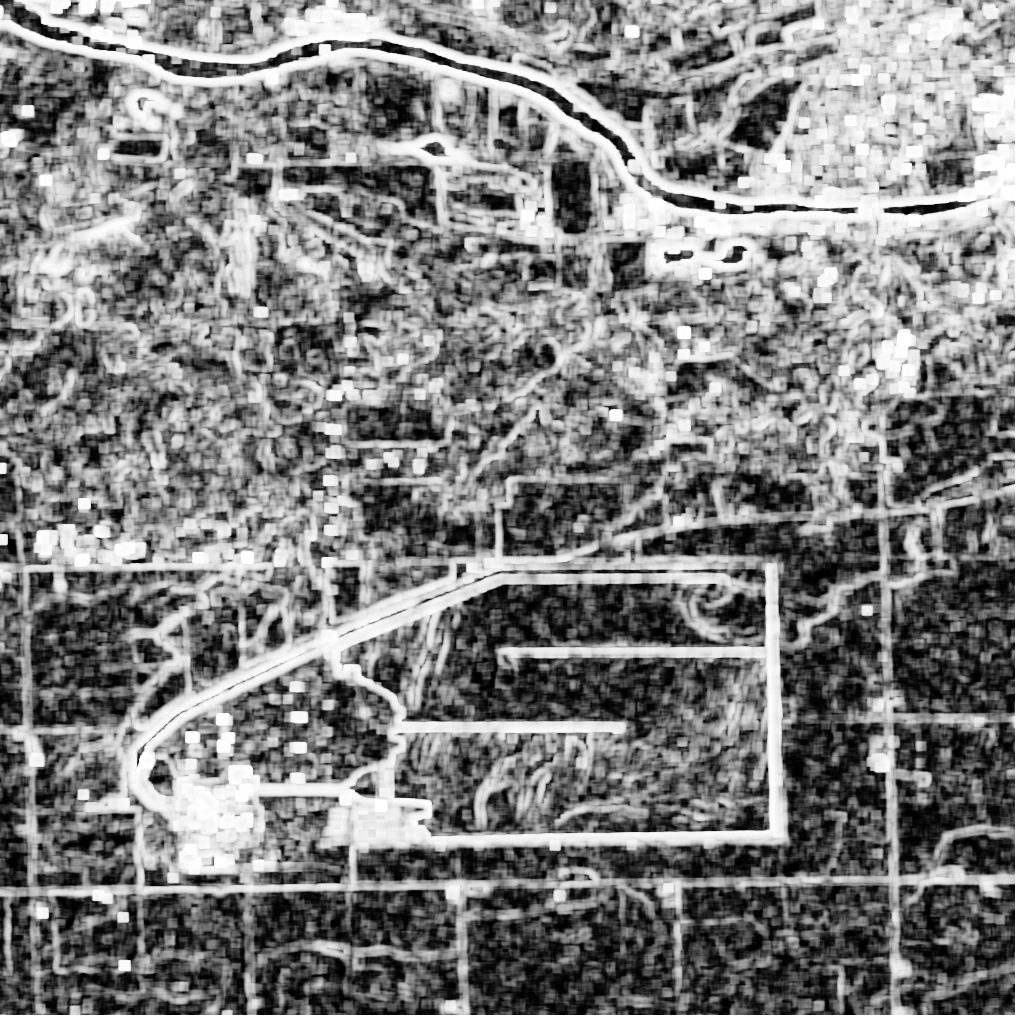
\includegraphics[width=\textwidth]{../../Figures/PNG/cv_Illinois_crops_1024}
    \caption{$T_\text{CV}$}
    \label{fig:real_images_test_Illinois-2}
  \end{subfigure}
  \hfill
  \begin{subfigure}[b]{0.3\textwidth}
    \centering
    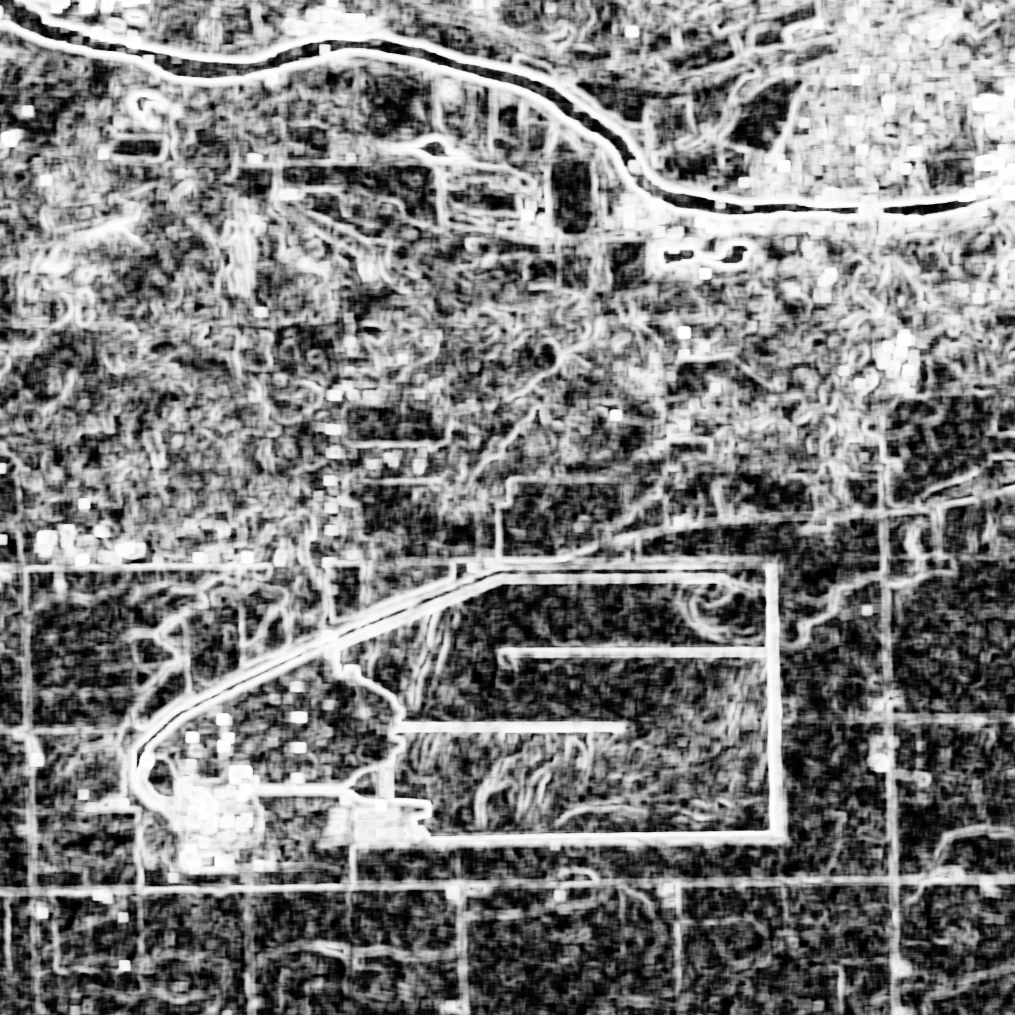
\includegraphics[width=\textwidth]{../../Figures/PNG/mnad_Illinois_crops_1024}
    \caption{$T_{\text{CV}_{\text{MnAD}}}$}
    \label{fig:real_images_test_Illinois-3}
  \end{subfigure}
  \caption{Results of applying the test statistics, Illinois-Region 2.}
  \label{fig:real_images_test_Illinois}
\end{figure}


\begin{figure}[H]
  \centering
  \begin{subfigure}[b]{0.3\textwidth}
    \centering
    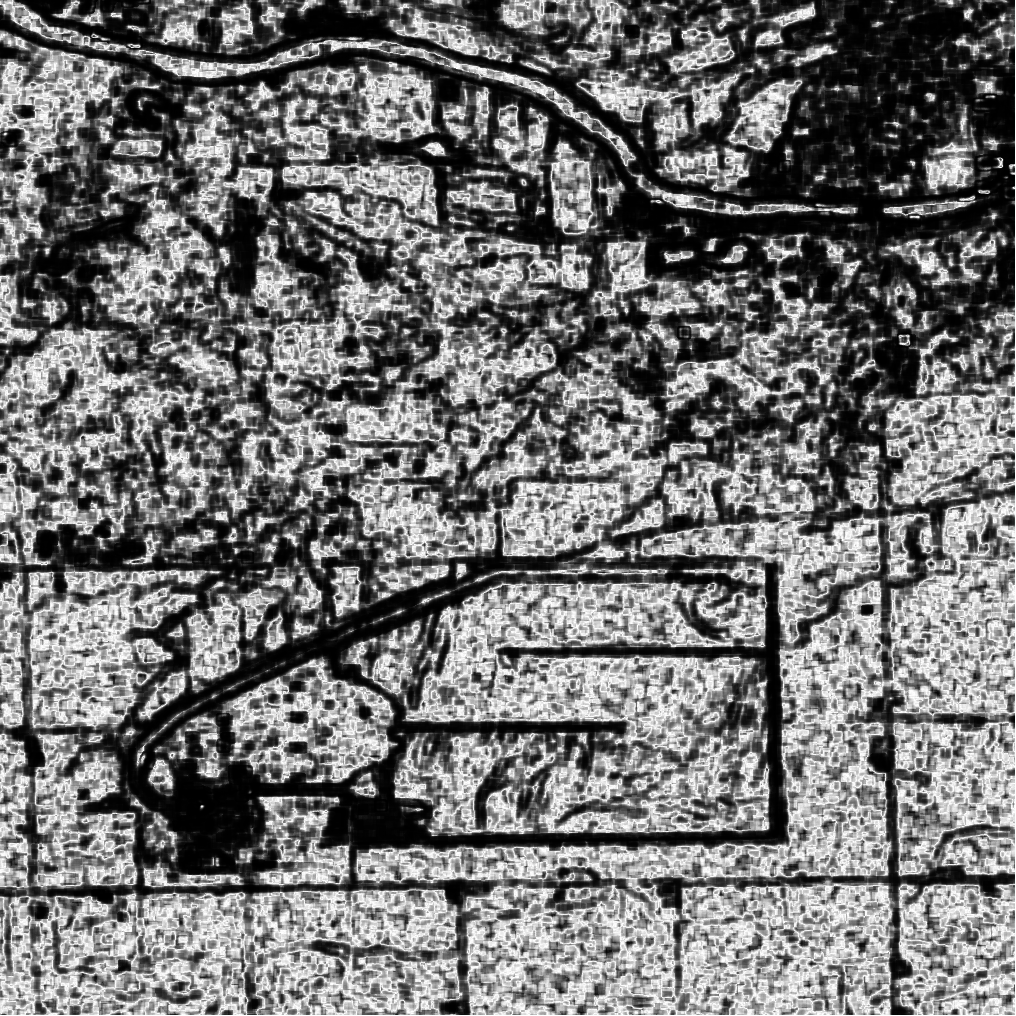
\includegraphics[width=\textwidth]{../../Figures/PNG/H_pvalue_Illinois_1024_36L_AO_200b}
    \caption{$S_{\widetilde{H}_{\text{AO}}}(\bm{Z}; L)$}
    \label{fig:Illinois_crops_pvalue-1}
  \end{subfigure}
  \hfill
  \begin{subfigure}[b]{0.3\textwidth}
    \centering
    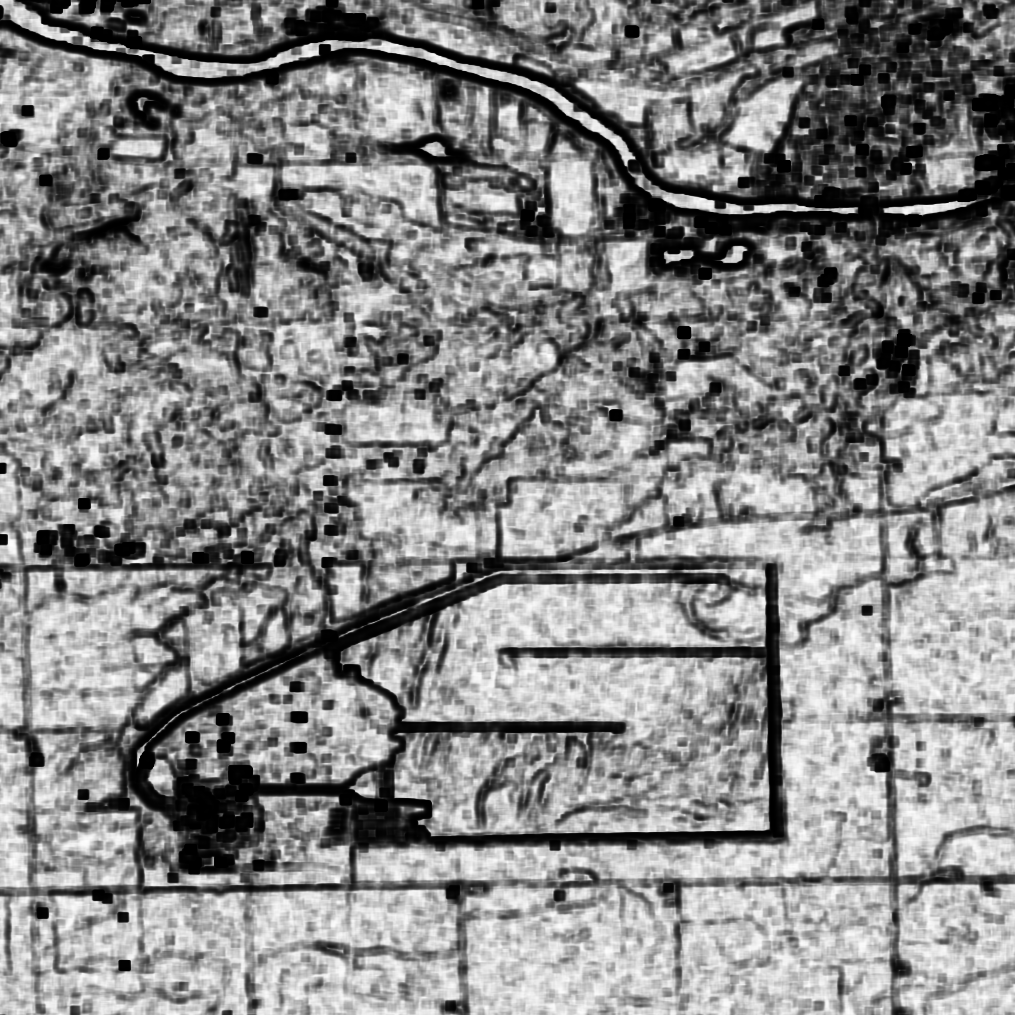
\includegraphics[width=\textwidth]{../../Figures/PNG/cv_pvalues_Illinois_crops_1024}
    \caption{$T_\text{CV}$}
    \label{fig:Illinois_crops_pvalue-2}
  \end{subfigure}
  \hfill
  \begin{subfigure}[b]{0.3\textwidth}
    \centering
    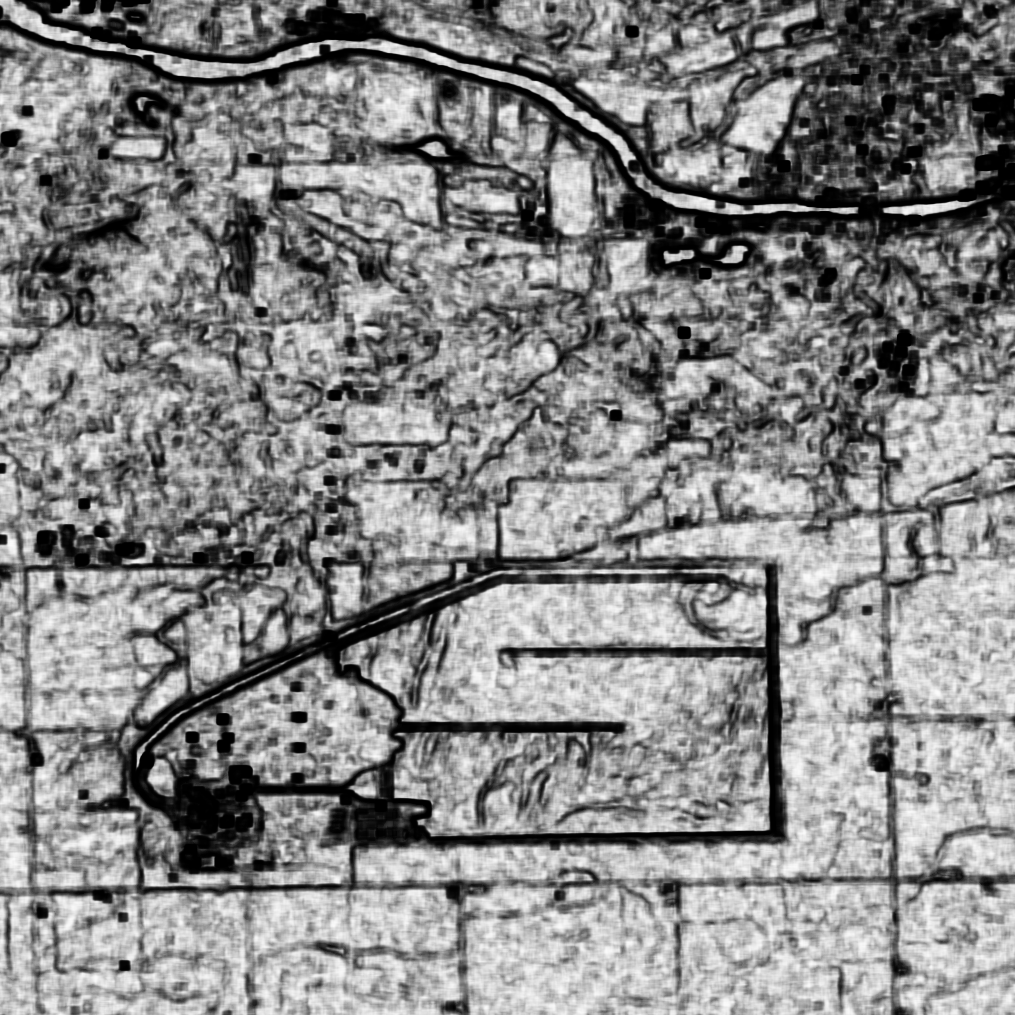
\includegraphics[width=\textwidth]{../../Figures/PNG/mnad_p_values_Illinois_crops_1024}
     \caption{$T_{\text{CV}_{\text{MnAD}}}$}
    \label{fig:Illinois_crops_pvalue-3}
  \end{subfigure}
  \caption{Map of $p$-values, Illinois-Region 2. }
  \label{fig:Illinois_crops_pvalue}
\end{figure}


\begin{figure}[H]
  \centering
  \begin{subfigure}[b]{0.3\textwidth}
    \centering
    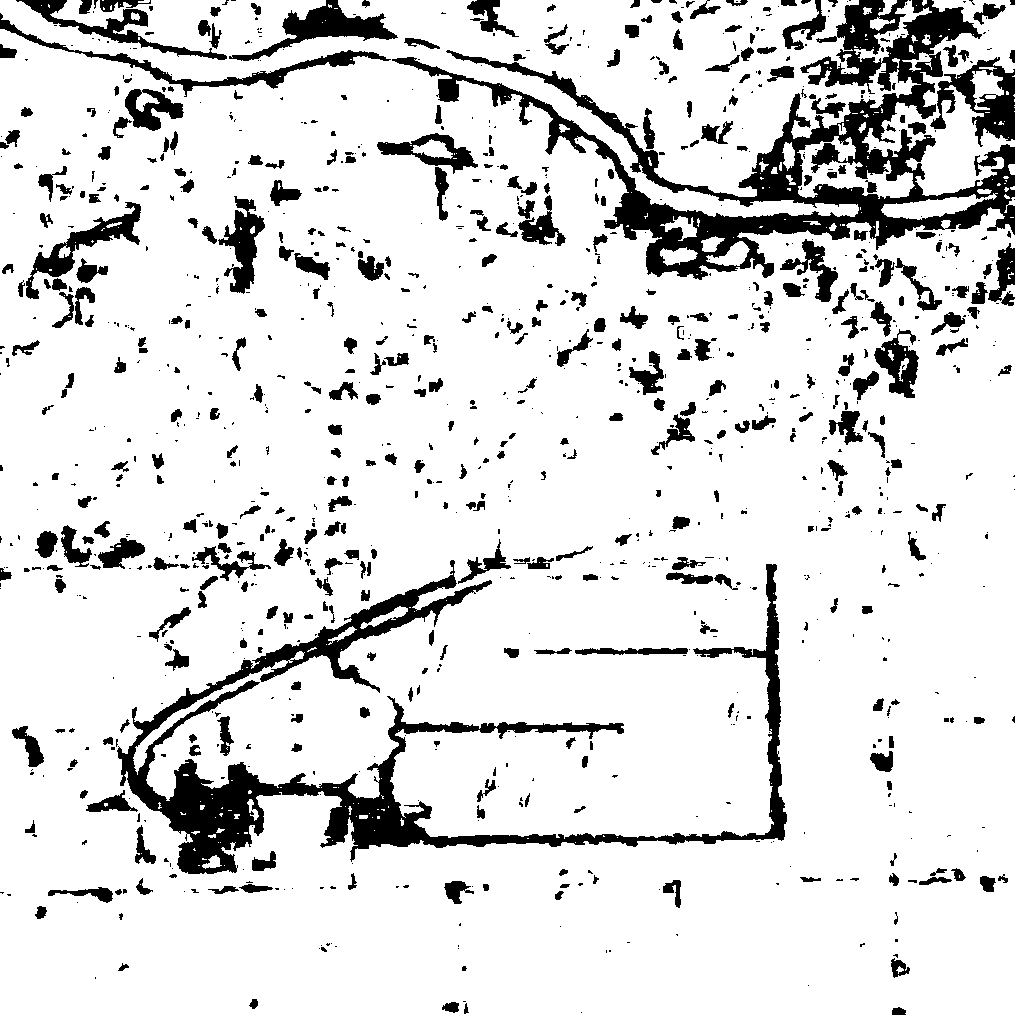
\includegraphics[width=\textwidth]{../../Figures/PNG/H_005_pvalues_Illinois_1024_36L_AO_200b}
    \caption{$S_{\widetilde{H}_{\text{AO}}}(\bm{Z}; L)$}
    \label{fig:Illinois_crops_0.05-1}
  \end{subfigure}
  \hfill
  \begin{subfigure}[b]{0.3\textwidth}
    \centering
    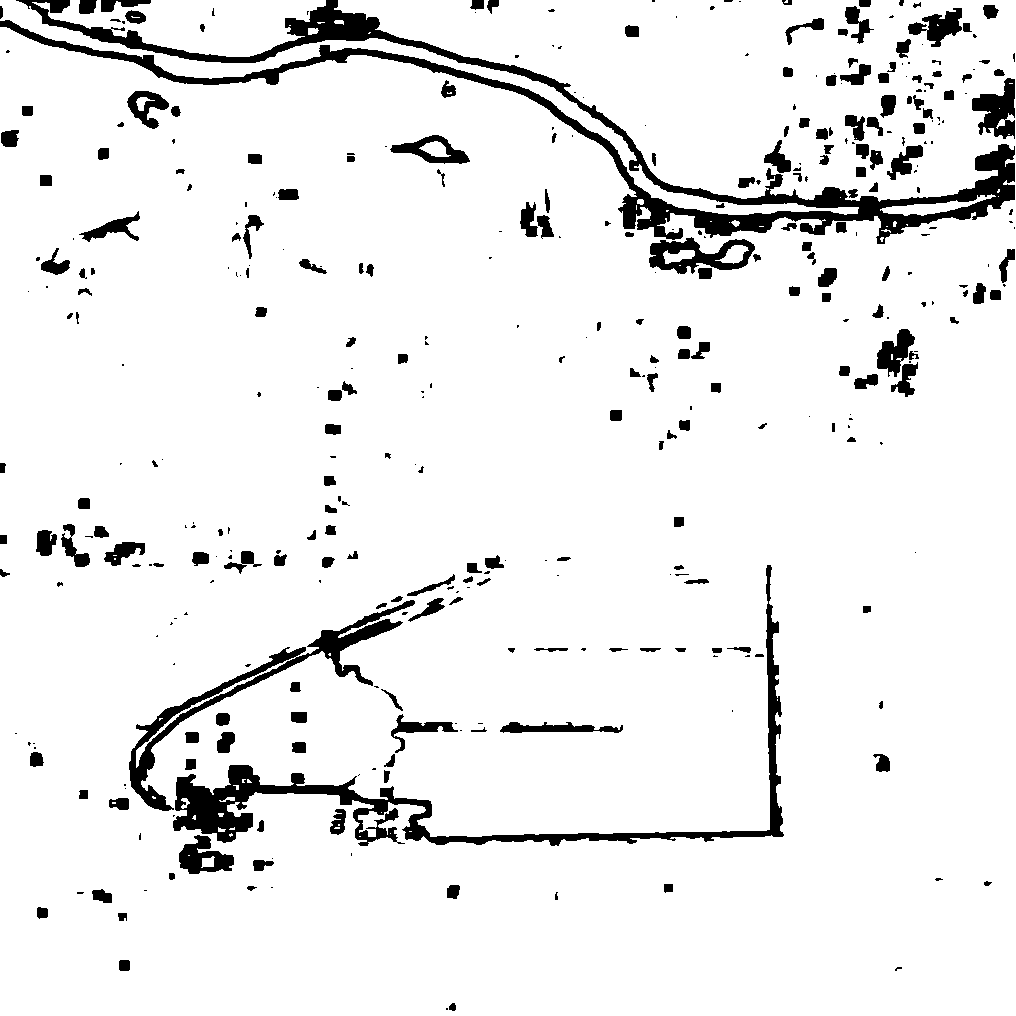
\includegraphics[width=\textwidth]{../../Figures/PNG/cv_005_pvalues_Illinois_crops_1024}
    \caption{$T_\text{CV}$}
    \label{fig:Illinois_crops_0.05-2}
  \end{subfigure}
  \hfill
  \begin{subfigure}[b]{0.3\textwidth}
    \centering
    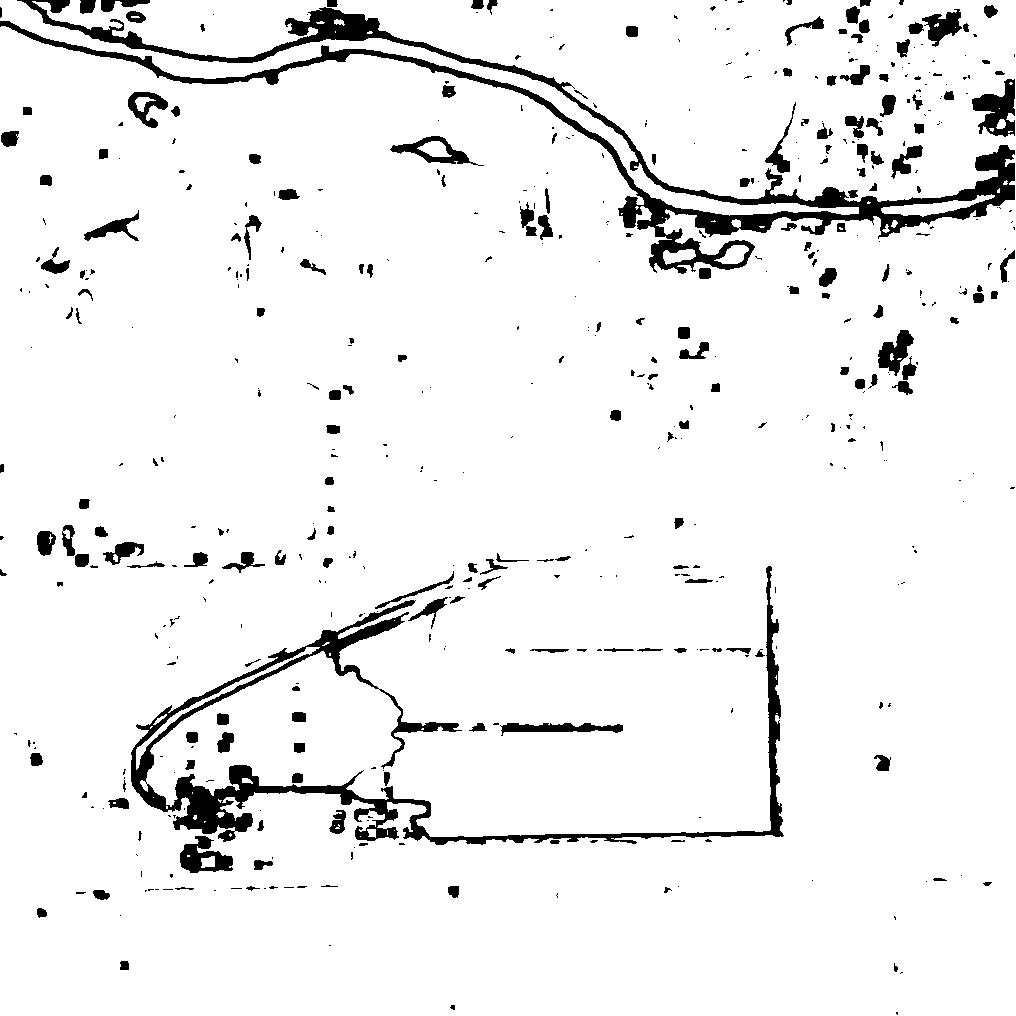
\includegraphics[width=\textwidth]{../../Figures/PNG/mnad_005_Illinois_crops_1024}
     \caption{$T_{\text{CV}_{\text{MnAD}}}$}
    \label{fig:Illinois_crops_0.05-3}
  \end{subfigure}
  \caption{Results for a threshold of $0.05$ of the $p$-value, Illinois-Region 2. }
  \label{fig:Illinois_crops_0.05}
\end{figure}



Using Shannon entropy is more meaningful than using the original and
robust CV to capture heterogeneity. It is justified that the dark areas
of the maps based on the \(T_\text{CV}\) and
\(T_{\text{CV}_{\text{MnAD}}}\) show coverage patterns similar to those
reported for the \(S_{\widetilde{H}_{\text{AO}}}(\bm{Z}; L)\) map. 
This suggests that although CV-based tests may produce slightly less
pronounced results than the entropy-based test, they still demonstrate a
comparable ability to detect heterogeneity within SAR images.

It is noticeable that the entropy and CV-based tools predicted
heterogeneity regions and boundaries where the statistical properties of
texture vary. The \(T_{\text{CV}_{\text{MnAD}}}\) test was shown to be
an effective edge detector. 
It emerges as a robust alternative to the classical CV test, making it less susceptible to the influence of
outliers and allowing it to produce more precise edges. 
Considering a
higher significance level may increase the sensitivity to edge detection
but also increase the risk of detecting false heterogeneous regions.

Additionally, assuming a \SI{5}{\percent} threshold for \(p\)-values, in
most cases, the heterogeneous regions detected by the
\(S_{\widetilde{H}{\text{AO}}}(\bm{Z}; L)\) test were more extensive
than those detected by the \(T_\text{CV}\) and
\(T_{\text{CV}_{\text{MnAD}}}\) tests. 
This was mainly observable in
Figures~\ref{fig:sim_SAR_Images_p05} \ref{fig:sim_SAR_Images_p05-1},
~\ref{fig:Mexico_crops_0.05} \ref{fig:Mexico_crops_0.05-1}, and~\ref{fig:lake_0.05} \ref{fig:lake_0.05-1}.
